\documentclass[11pt]{article}
\newcommand{\DocTitle}{Architecture and Pattern Crosswalk}
\newcommand{\DocSubtitle}{DDD, microfrontends, microservices and contract-driven composition}
\newcommand{\DocID}{DOS-03}
% design-of-sites-style.tex
% Suite preamble for the Web Design Patterns / Design of Sites suite.
%
% RECONSTRUCTION PROVENANCE: the nine uploaded suite documents load a shared
% preamble with `\input{style.tex}`, but no `style.tex` was present in the
% upload batches or anywhere in this repository's history. This file is a
% documented, suite-specific reconstruction inferred from the interface the
% documents actually use: per-document metadata (\DocTitle, \DocSubtitle,
% \DocID defined before this file is input), the front-matter renderer
% \MakeFront, the provenance marker \Provenance, the callout environments
% groundedbox/modernbox/notebox/decisionbox, and the colors
% Ink/Ocean/Mint/Amber/Faint referenced in document TikZ code. It is NOT the
% recovered original style; the original visual design is unknown.
%
% pdfLaTeX only.
\usepackage[T1]{fontenc}
\usepackage[utf8]{inputenc}
\usepackage{lmodern}
\usepackage{microtype}
\usepackage[letterpaper,margin=0.85in,headheight=15pt]{geometry}
\usepackage[table]{xcolor}
\definecolor{Ink}{HTML}{1E2A36}
\definecolor{Ocean}{HTML}{0F4C72}
\definecolor{Mint}{HTML}{0E7E6B}
\definecolor{Amber}{HTML}{B07A1E}
\definecolor{Faint}{HTML}{F2F7F9}
\usepackage{amsmath,amssymb}
\usepackage{array,booktabs,longtable,tabularx,multirow}
\usepackage{enumitem}
\usepackage[most]{tcolorbox}
\usepackage{listings}
\usepackage{tikz}
\usetikzlibrary{arrows.meta,positioning,shapes.geometric,fit,calc}
\usepackage{needspace}
\usepackage{titlesec}
\usepackage{fancyhdr}
\usepackage{lastpage}
\usepackage{xurl}
\usepackage{hyperref}
\hypersetup{colorlinks=true,linkcolor=Ocean,urlcolor=Mint,citecolor=Ocean,pdftitle={\DocTitle},pdfauthor={Web Design Patterns Engineering Suite}}
\setlength{\parindent}{0pt}
\setlength{\parskip}{5pt plus 1pt}
\setlength{\emergencystretch}{2em}
\renewcommand{\arraystretch}{1.18}
\setlist[itemize]{itemsep=2pt,topsep=3pt,leftmargin=1.5em}
\setlist[enumerate]{itemsep=2pt,topsep=3pt,leftmargin=1.7em}
\titleformat{\section}{\Large\bfseries\color{Ocean}}{\thesection}{0.7em}{}[\vspace{-3pt}\color{Mint}\titlerule]
\titleformat{\subsection}{\large\bfseries\color{Ink}}{\thesubsection}{0.6em}{}
\titleformat{\subsubsection}{\normalsize\bfseries\color{Mint}}{\thesubsubsection}{0.55em}{}
\pagestyle{fancy}
\fancyhf{}
\fancyhead[L]{\sffamily\footnotesize\color{Ocean} Design of Sites | \DocID}
\fancyhead[R]{\sffamily\footnotesize\color{Ink} Web Design Patterns Suite}
\fancyfoot[L]{\sffamily\scriptsize Original interpretive guidance; pattern names used as a taxonomy}
\fancyfoot[R]{\sffamily\scriptsize\thepage\ / \pageref{LastPage}}
\renewcommand{\headrulewidth}{0.3pt}
\lstdefinestyle{dositescode}{basicstyle=\ttfamily\footnotesize,breaklines=true,columns=fullflexible,keepspaces=true,showstringspaces=false,frame=single,rulecolor=\color{Mint},backgroundcolor=\color{Faint},aboveskip=8pt,belowskip=8pt}
\lstset{style=dositescode}
% Callouts. groundedbox marks statements verified against the public
% bibliographic record; modernbox marks newly authored modern engineering
% interpretation; notebox is a study/summary callout; decisionbox records
% decisions and trade-offs.
\newtcolorbox{groundedbox}[1][]{enhanced,breakable,colback=Faint,colframe=Mint,boxrule=0.5pt,arc=1.5mm,title={Grounded in the public record},fonttitle=\bfseries\small,#1}
\newtcolorbox{modernbox}[1][]{enhanced,breakable,colback=white,colframe=Ocean,boxrule=0.5pt,arc=1.5mm,title={Modern engineering interpretation},fonttitle=\bfseries\small,#1}
\newtcolorbox{notebox}[1][]{enhanced,breakable,colback=Faint,colframe=Amber,boxrule=0.5pt,arc=1.5mm,#1}
\newtcolorbox{decisionbox}[1][]{enhanced,breakable,colback=white,colframe=Amber,boxrule=0.5pt,arc=1.5mm,title={Decision record},fonttitle=\bfseries\small,#1}
% Front matter renderer: consumes \DocTitle, \DocSubtitle, \DocID.
\newcommand{\MakeFront}{%
  \thispagestyle{empty}%
  {\color{Mint}\rule{\textwidth}{3pt}}\par\vspace{16pt}
  {\sffamily\small\color{Amber}\bfseries \DocID\par}\vspace{10pt}
  {\Huge\bfseries\color{Ocean} \DocTitle\par}\vspace{12pt}
  {\Large\color{Ink} \DocSubtitle\par}\vspace{14pt}
  {\small\color{Ink} Independent educational and engineering companion to \emph{The Design of Sites} (2nd edition). Original explanatory material; the copyrighted pattern text is not reproduced.\par}
  \vspace{10pt}{\color{Mint}\rule{\textwidth}{1pt}}\par\vspace{8pt}
  \tableofcontents\clearpage}
% Provenance marker used at the top of each document body.
\newcommand{\Provenance}{\par\noindent{\footnotesize\sffamily\color{Amber}\bfseries Provenance:}~{\footnotesize\color{Ink}\itshape claims grounded in the public bibliographic record are boxed and cited; everything else is newly authored interpretation.}\par\smallskip}

\begin{document}
\MakeFront
\section{Architecture mapping principles}

\Provenance
\begin{groundedbox}The book organizes interface-design concerns into 13 pattern groups [B1]. The architectural mapping in this document is a modern, author-created crosswalk, not part of the 2006 book.\end{groundedbox}
\begin{modernbox}Model a site as user journeys operating across presentation, domain/application capabilities, data contracts, security control planes and delivery infrastructure. A pattern group can constrain several layers without defining service boundaries by itself.\end{modernbox}

\section{A--M crosswalk}
\begin{longtable}{@{}p{15mm}p{29mm}p{54mm}p{44mm}@{}}\toprule\textbf{Group}&\textbf{Architectural lens}&\textbf{Modern responsibility}&\textbf{Evidence artifact}\\\midrule\endhead
A & Domain discovery & Domain boundaries and user missions & Context map; domain glossary\\
B & Information architecture & Route contracts and taxonomy ownership & Sitemap; routing rules\\
C & Experience composition & Shell and entry-point orchestration & Homepage experiment and route metrics\\
D & Content platform & Schema versioning and publishing workflow & CMS contracts; content lifecycle\\
E & Trust and policy & Identity, privacy and policy enforcement & Threat model; privacy controls\\
F & Commerce domain & Cart, checkout, payment and order commands & Saga/idempotency tests\\
G & Relevance and social domain & Recommendation, review and consent models & Bias/abuse test suite\\
H & Workflow application & State machines and authentication lifecycle & Task and recovery tests\\
I & Design system & Responsive tokens and presentation semantics & Visual regression and zoom tests\\
J & Search domain & Index freshness, relevance and ACL filtering & Search evaluation dataset\\
K & Navigation design system & Shared accessible navigation components & Keyboard and screen reader tests\\
L & Performance platform & Caching, streaming, asset delivery and monitoring & RUM budget and tracing\\
M & Mobile experience & Responsive inputs, offline behavior and permissions & Mobile device matrix\\
\bottomrule\end{longtable}
\section{Reference capability architecture}

\begin{center}
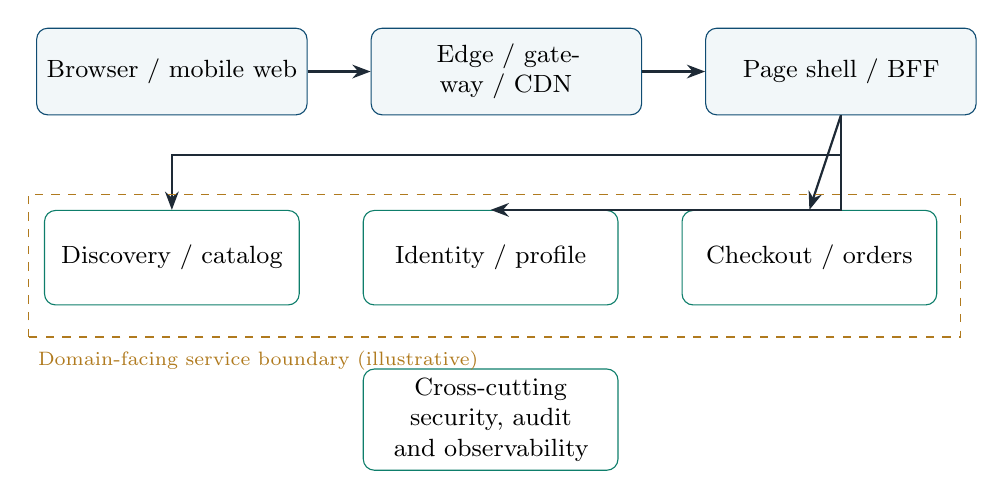
\begin{tikzpicture}[node distance=7mm and 8mm,box/.style={draw=Ocean,rounded corners,fill=Faint,text width=32mm,minimum height=11mm,align=center,font=\small},svc/.style={draw=Mint,rounded corners,fill=white,text width=30mm,minimum height=12mm,align=center,font=\small},arr/.style={-Stealth,thick,draw=Ink}]
\node[box] (browser) {Browser / mobile web};
\node[box,right=of browser] (edge) {Edge / gateway / CDN};
\node[box,right=of edge] (shell) {Page shell / BFF};
\node[svc,below=12mm of browser] (catalog) {Discovery / catalog};
\node[svc,right=of catalog] (identity) {Identity / profile};
\node[svc,right=of identity] (orders) {Checkout / orders};
\node[svc,below=8mm of identity] (policy) {Cross-cutting security, audit and observability};
\draw[arr] (browser)--(edge);\draw[arr] (edge)--(shell);
\draw[arr] (shell.south) -- ++(0,-5mm) -| (catalog.north);
\draw[arr] (shell.south) -- (orders.north);
\draw[arr] (shell.south) |- (identity.north);
\draw[dashed,draw=Amber] ($(catalog.south west)+(-2mm,-4mm)$) rectangle ($(orders.north east)+(3mm,2mm)$);
\node[font=\scriptsize,anchor=west,text=Amber] at ($(catalog.south west)+(-2mm,-7mm)$) {Domain-facing service boundary (illustrative)};
\end{tikzpicture}
\end{center}
\textbf{Read as a logical view, not a deployment prescription.} The BFF (backend for frontend) may be omitted if the team has one cohesive web application and direct contracts remain safe and comprehensible. Cross-cutting controls must be implemented at each applicable trust boundary, not delegated to the diagram.

\section{Bounded contexts and ownership}

\begin{tabularx}{\linewidth}{@{}p{30mm}p{32mm}XX@{}}\toprule
Context & Domain authority & User-facing capability & Integration contract\\\midrule
Identity & Accounts, sessions & Sign in, recovery & OIDC/OAuth-based integration as applicable; session lifecycle\\
Catalog & Products, categorization & Browse and detail & Versioned read API and publication events\\
Search & Index and ranking policy & Query, filter & ACL-aware search API; index change feed\\
Commerce & Cart and order intents & Checkout & Idempotent commands; price validation\\
Payment & Payment state integration & Tender & Tokenized PSP integration; webhooks\\
Content & Content and localization & Publishing & Content schema and revision API\\
Privacy & Data rights and purposes & Preferences & Consent events and policy checks\\
\bottomrule\end{tabularx}
\begin{decisionbox}A page, pattern or component is \emph{not} automatically a microservice. Prefer bounded contexts derived from domain semantics, transaction ownership and team capabilities.\end{decisionbox}

\section{Microfrontend adoption decision}

\textbf{Default:} one cohesive frontend with modular domain packages. Separate frontends only when distinct teams need independent deployment and the value exceeds shared-runtime, design consistency, bundle and operational costs [S11].
\begin{enumerate}
\item Establish domain slices with stable routing and API contracts.
\item Decide composition model: server-side fragments, build-time packages, route-level applications, or runtime federation.
\item Keep authentication, navigation, accessibility and observability contracts under an explicit shared platform owner.
\item Version shared dependencies carefully; avoid duplicate heavy runtimes and competing CSS globals.
\item Implement progressive rollout and rollback by slice; monitor cross-slice journeys end to end.
\end{enumerate}
\textbf{Reject the split} if independent deployment is not required, performance is already fragile or the team cannot own cross-boundary incidents.

\section{Example: browse-to-buy end-to-end journey}

\textbf{Patterns.} B4 task organization; F2 product details; F3 cart; F6 payment; F8 order confirmation; H1 process funnel; E6 secure connections; K13 meaningful errors; L6 fast content.
\begin{enumerate}
\item Customer enters the product route (shell owns route and landmarks).
\item Catalog resolves product data; price and inventory are displayed with explicit source metadata.
\item Cart service validates item IDs, quantity, unit price source and availability.
\item Checkout command takes an idempotency key and expected cart version.
\item Payment provider supplies a token and independently confirms settlement status.
\item Orders persist a state transition and publish an event once; duplicate callbacks are safely ignored.
\item Confirmation is accessible and recoverable, even after a network interruption.
\end{enumerate}
\textbf{Failure path.} If price or stock changes, do not charge silently. Return a recoverable state and require explicit reapproval of material changes.

\section{API contract sketch (illustrative)}

\begin{lstlisting}[language={},caption={OpenAPI fragment -- add security schemes and full error schemas for production}]
openapi: 3.1.1
info: { title: Checkout API, version: 1.0.0 }
paths:
  /checkout/confirm:
    post:
      operationId: confirmCheckout
      parameters:
        - name: Idempotency-Key
          in: header
          required: true
          schema: { type: string, minLength: 16 }
      requestBody:
        required: true
        content:
          application/json:
            schema:
              type: object
              required: [cartId, expectedVersion]
              properties:
                cartId: { type: string }
                expectedVersion: { type: integer, minimum: 0 }
      responses:
        '201': { description: Order created }
        '409': { description: Cart changed; customer must review }
        '422': { description: Business validation failed }
\end{lstlisting}
\textbf{Note:} Validate cart ownership and final totals on the server; the idempotency key alone is not an authorization mechanism. See [S7--S8].

\section{Architecture decision rubric}

\begin{tabularx}{\linewidth}{@{}p{38mm}XX@{}}\toprule
Question & Favor modular monolith & Consider distributed boundary\\\midrule
Independent deployment & Not required & Required across autonomous teams\\
Data consistency & Strong transaction locality & Eventual consistency acceptable\\
Operational maturity & Limited incident/on-call coverage & Dedicated ownership and observability\\
Traffic/scale & Similar scaling profile & Uneven or independently scaling workloads\\
Security & Simpler trust model desired & Control segmentation adds material value\\
UX cohesion & Frequent shared-state transitions & Coarse-grained journeys; stable contracts\\
\bottomrule\end{tabularx}


\clearpage
% design-of-sites-references.tex
% Shared references section for the Web Design Patterns / Design of Sites
% suite.
%
% RECONSTRUCTION PROVENANCE: the nine uploaded suite documents end with
% `\input{references.tex}`, but no `references.tex` was present in the upload
% batches or anywhere in this repository's history. The documents cite only
% keys [B1] and [B2] (bracketed tokens such as "[B4, F1, H10, ...]" are
% pattern-ID template placeholders, not citations). The two entries below are
% reconstructed from the bibliographic facts the documents themselves state:
% publisher record and bibliographic-database record of the second edition.
% This file is NOT the recovered original reference list.
\clearpage
\section*{References}
\begin{description}[leftmargin=3.2em,style=nextline]
  \item[{[B1]}] Publisher bibliographic record and public table of contents:
    D.~K.~van Duyne, J.~A.~Landay, J.~I.~Hong, \emph{The Design of Sites:
    Patterns, Principles, and Processes for Crafting a Customer-Centered Web
    Experience}, 2nd edition, Prentice Hall, December 2006, 1{,}024 pages.
    Confirms the five foundational chapters, the thirteen pattern groups
    (A--M), the 107 pattern labels and the research appendixes used as this
    suite's taxonomy.
  \item[{[B2]}] Bibliographic-database record (O'Reilly learning-platform
    catalog entry) for the same second edition; corroborates edition,
    authors, publication date and chapter/group structure. The copyrighted
    pattern explanations themselves were not retrieved or reproduced for
    this suite.
\end{description}

\end{document}
